% Self-contained source composed from pinned proofs and measured outputs.
\documentclass[12pt]{article}
\usepackage[letterpaper,margin=1in]{geometry}
\usepackage[T1]{fontenc}
\usepackage{newtxtext,ragged2e}
\usepackage[justification=raggedright,singlelinecheck=false]{caption}
\usepackage{amsmath,amssymb,amsthm,booktabs,array}
\usepackage{tikz}
\usepackage[authoryear,round]{natbib}
\usepackage[hidelinks]{hyperref}
\usepackage{xurl,microtype,placeins}
\usepackage[mathlines]{lineno}
\AtBeginDocument{\raggedright\linenumbers}
\setlength{\emergencystretch}{2em}
\renewcommand{\topfraction}{0.95}
\renewcommand{\bottomfraction}{0.9}
\renewcommand{\textfraction}{0.05}
\renewcommand{\floatpagefraction}{0.75}
\newtheorem{theorem}{Theorem}
\newtheorem{proposition}{Proposition}
\newtheorem{corollary}{Corollary}
\newcommand{\F}{\mathcal{F}}
\newcommand{\R}{\mathbb R}
\newcommand{\M}{\mathcal M}
\newcommand{\Oset}{\mathcal O}
\newcommand{\clip}{\operatorname{clip}}
\title{Adaptive Reading Budgets for Joint Forecast Audits with Cumulative Data}
\author{Jishan Kapoor\\Independent Researcher\\Toronto M4Y 1C9, Canada\\
Corresponding author: \href{mailto:kapoorjishan19@gmail.com}{kapoorjishan19@gmail.com}}
\date{}
\begin{document}
\maketitle
\begin{abstract}
\textbf{Background.} Model audits share verification readings across several
predictors. We ask how many readings suffice for precise comparisons and
when choosing later readings after earlier answers reduces this requirement.

\textbf{Methods.} We study sharp intervals for affine model-loss contrasts
on compact convex sets using a finite query dictionary. We prove fixed-budget
bounds, compute minimum fixed reading budgets, and replay certified policies
on cumulative-meter data.

\textbf{Results.} For one comparison, if a deterministic policy guarantees
precision with two exact scalar readings, some randomized fixed batch succeeds with
worst-case probability at least $1/2$. This lower bound disappears with two
comparisons. For every $m\geq3$, we construct instances where adaptation
always succeeds but the best randomized batch succeeds with worst-case
probability exactly $1/m$. All coordinates are queryable, the budget remains
two, and each comparison is separately certifiable by a fixed batch.
The separation also holds for all pairwise comparisons among three models.
On 225 of 1,098 meter blocks across six systems, two adaptive readings
guarantee halving every comparison's width, while the minimum fixed budget
is three. Of these, 222 have optimal randomized two-reading batch success
exactly $1/2$. The one-third reading reduction on qualifying blocks becomes
6.40\% and 7.67\% across the complete original and external panels.
Capacity information reduces the advantage, and measured public-API retrieval
favors bulk.

\textbf{Conclusions.} Sharing a reading budget can make feedback necessary
for assurance even when separate comparisons need none. The construction
proves a fixed-budget boundary; the retrospective meter study quantifies
its narrower benefit in required readings, separately from retrieval cost.
\end{abstract}
\noindent\textbf{Keywords:} artificial intelligence; machine learning;
adaptive information; minimax risk; optimal recovery; robust optimization.

\section{Introduction}
A model audit may need more verification data before it can report a precise
comparison. The auditor can retrieve a complete record, choose a batch of
readings, or choose later readings after seeing earlier answers. We study
this last option, adaptive querying. Our output is a sharp interval: the
smallest interval containing the loss difference for every record compatible
with the observations. Its width measures how much the reported comparison
can still change. We ask when feedback is needed to meet a stated width
requirement with the same reading budget.

This is an acquisition problem for fixed predictors. The auditor specifies
which loss contrasts must be precise, what information is already available,
and which measurements may be requested. We first compute the smallest
sufficient fixed reading budget, then test whether two adaptive readings
can reduce it. The algorithm returns a reading plan and checks its intervals.
Identifying a better model is a separate
condition: a comparison interval must also exclude zero.

% Native TikZ overview. No extra TikZ libraries or external image files.
% Scope: uncapped exact-total simplex; noiseless internal prefix readings.
\begin{figure}[htbp]
\centering
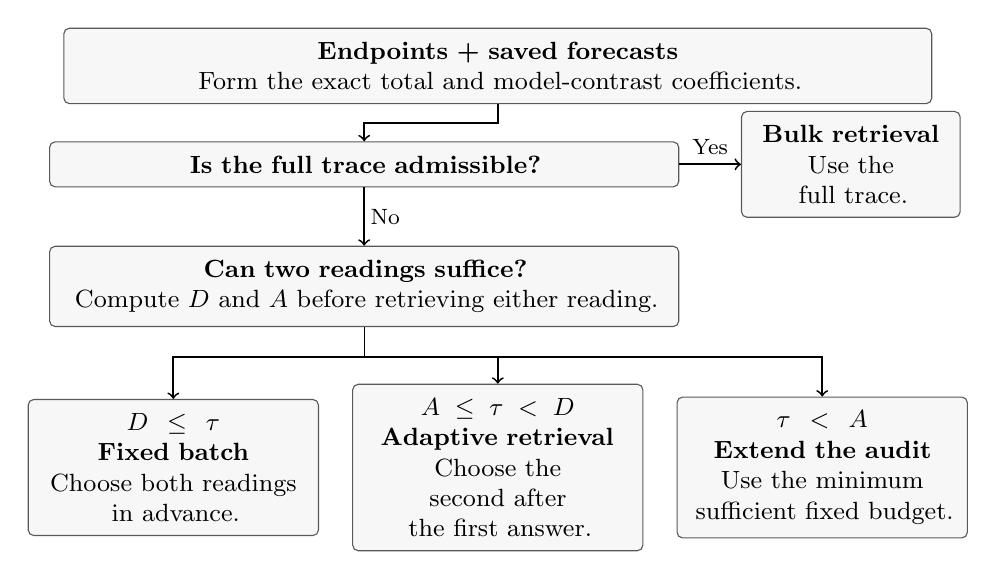
\begin{tikzpicture}[x=0.01\linewidth,y=1cm,
  every node/.style={font=\small,align=center},
  flowbox/.style={draw=black!65,rounded corners=2pt,fill=black!3,
    inner sep=5pt},
  flowarrow/.style={->,line width=0.65pt}]
\node[flowbox,text width=0.88\linewidth] (inputs) at (50,0)
  {\mbox{\textbf{Endpoints + saved forecasts}}\\
   Form the exact total and model-contrast coefficients.};
\node[flowbox,text width=0.63\linewidth] (access) at (36,-1.25)
  {\mbox{\textbf{Is the full trace admissible?}}};
\node[flowbox,text width=0.20\linewidth] (bulk) at (87,-1.25)
  {\mbox{\textbf{Bulk retrieval}}\\Use the full trace.};
\node[flowbox,text width=0.63\linewidth] (plan) at (36,-2.80)
  {\mbox{\textbf{Can two readings suffice?}}\\
   Compute $D$ and $A$ before retrieving either reading.};
\node[flowbox,text width=0.275\linewidth] (fixed) at (16,-5.10)
  {$D\leq\tau$\\\mbox{\textbf{Fixed batch}}\\
   Choose both readings\\in advance.};
\node[flowbox,text width=0.275\linewidth] (adaptive) at (50,-5.10)
  {$A\leq\tau<D$\\\mbox{\textbf{Adaptive retrieval}}\\
   Choose the second after\\the first answer.};
\node[flowbox,text width=0.275\linewidth] (escalate) at (84,-5.10)
  {$\tau<A$\\\mbox{\textbf{Extend the audit}}\\
   Use the minimum\\sufficient fixed budget.};
\draw[flowarrow] (inputs.south) -- (50,-0.72) -- (36,-0.72)
  -- (access.north);
\draw[flowarrow] (access.east) -- node[above,font=\footnotesize]{Yes}
  (bulk.west);
\draw[flowarrow] (access.south) -- node[midway,right,inner sep=2pt,font=\footnotesize]{No}
  (plan.north);
\draw (plan.south) -- (36,-3.70) -- (50,-3.70);
\draw[flowarrow] (50,-3.70) -- (16,-3.70) -- (fixed.north);
\draw[flowarrow] (50,-3.70) -- (adaptive.north);
\draw[flowarrow] (50,-3.70) -- (84,-3.70) -- (escalate.north);
\end{tikzpicture}
\caption{Choosing an audit protocol. For the exact-total, noiseless prefix
model, let $J_Q=\max_r W_{r,Q}/W_{r,0}$ over contrasts with positive initial
width. Let $D=\min_Q\sup_y J_Q(y)$ and
$A=\min_{P\,\mathrm{det.\ adaptive}}\sup_y J_{Q_P(y)}(y)$ under the same
two-reading budget. We fix the target $\tau$ before retrieval; the main
application uses $\tau=1/2$. Since $A\leq D$, the three restricted-access
branches exhaust the possibilities for two-reading certainty, including randomized
policies (Proposition~\ref{prop:assurance-feasibility}). Their optimal
success probabilities below one are assessed separately. The fixed-budget
calculation in Section~\ref{sec:minimum-fixed-budget} supplies an explicit
fallback when two readings cannot guarantee success. Bulk is preferred on the measured public
API when its full response is admissible (Section~\ref{sec:actual-api}).}
\label{fig:audit-workflow}
\end{figure}

The central result is a boundary between one comparison and a shared
collection of comparisons. For one affine contrast, a deterministic policy
that guarantees precision with two exact scalar readings implies a
randomized fixed batch with worst-case success at least one half
(Theorem~\ref{thm:helly-precision}). With two contrasts, that floor disappears.
For every $m\geq3$, Theorem~\ref{thm:two-target-collapse} constructs instances
with optimal adaptive success $1$ and optimal batch success $1/m$, still
using two readings. Each contrast separately has a successful fixed batch;
all coordinates are queryable at equal cost. The same separation holds for
all pairs among three nonnegative forecast vectors
(Corollary~\ref{cor:all-pairs-collapse}). The dictionary grows with $m$,
and three fixed queries suffice. Moreover, the optimal batch mixture is
unique: it assigns mass $1/m$ to each of $m$ necessary batches. Even positive
worst-record success requires all $m$ batches. This exact support requirement
isolates what fails when separately sufficient measurements share a budget.

We make that distinction computable for cumulative-meter audits. An exact
two-query planner and matching certificates identify 165 of 819 original
blocks and 57 of 279 external blocks where feedback guarantees precision
for all six model pairs, while the best randomized batch succeeds with
worst-case probability exactly one half. Complete-panel replay then measures
what the policies achieve on the stored answers. We also determine the
minimum fixed reading budget: 168 original and 57 external blocks require
three fixed readings but only two adaptive readings. Thus the application
measures the readings needed for assurance. We compare this requirement with
the retrieval interface in a separate public-API control.

The same calculation can rule out an insufficient budget. Explicit adverse
records show that randomizing an adaptive policy cannot restore certainty
on any of the 583 blocks without a deterministic guarantee
(Proposition~\ref{prop:assurance-feasibility}). Thus the method supports a
three-way decision: choose a fixed batch, use feedback, or obtain more
information.

The paper develops the scalar bound, the shared-budget construction and the
meter planner, then reports its certificates, recorded outcomes and controls.
The retrospective study reuses frozen source panels. Online Resource~1
retains the supporting scalar penalty classification (S11), a separate
mean-joint-width construction (S14), historical controls and executable
source-to-table verification.

\subsection{Related work and the contribution boundary}
Partial identification studies conclusions that survive incomplete
observations \citep{manski,polo}. Cancellation in paired squared losses
already yields an affine function of the missing truth \citep{patton}.
Active evaluation and model selection acquire labels to estimate performance
or choose predictors \citep{sawade,hara,active,okanovic2025}. We instead
require the entire compatible interval of each fixed-record contrast to
meet a declared precision target. \citet[Theorem~1 and Proposition~1]{kuboyama2026}
studies completion-based model-choice certificates with adaptive binary
labels and shared paired bounds. Its distinction between hindsight certificate
size and acquisition requirements (Theorem~2 and Proposition~3) is also
relevant here; our guarantees concern joint widths for continuous targets.

The width of an information fiber is the established local diameter of
information \citep[Section~4.1]{novak2008}. Our shared objective is its
weighted $\ell_\infty$ version for a vector target. Classical deterministic
adaptivity bounds cover linear information on convex symmetric classes
\citep[Theorems~4.4--4.5]{novak2008}; nonsymmetric recovery is studied by
\citet{novak1995}, and noisy scalar criteria by
\citet[Theorems~2--3 and~5]{osipenko}. Modern randomized recovery minimizes
reconstruction error \citep[Section~2 and Proposition~4.1]{krieg2025}
\citep[Section~9.1, Eq.~(9.15), author manuscript v2]{krieg2026}.
Our precision objective instead asks whether the full terminal fiber is
sufficiently narrow. For supporting mean-width results, the order of the
worst-record and randomization operations also differs from expected global
radius \citep[Eq.~(2.4), Remark~6.1, author manuscript v2]{krieg2026}.
Online Resource~1, S11 gives that comparison and the scalar penalty
classification, whose sufficient direction applies Sion's minimax theorem
\citep[Theorem~3.4]{sion1958} and Jensen's inequality.

Information-dependent decisions are established in adjustable robust
optimization \citep{wei2024,ddid}. Our scalar precision bound adapts the
sufficient-policy result of \citet[Theorem~2 and Example~5]{kurtz2026}.
Kurtz's Theorem~11 also permits policy counts to grow with recourse-region
complexity. In our construction, each scalar conditional width is affine,
but their joint maximum loses the concavity used by the scalar bound.
We realize that obstruction with actual coordinate-query fibers: two
affine targets and two unit-cost readings have exact success values $1$
and $1/m$, although each target alone has a sufficient fixed batch.
The adverse records further force support $m$ for any positive batch
success and uniquely determine the optimal mixture. The output dimension
and budget stay fixed while the measurement dictionary grows. This is the
specific contribution beyond general policy-count bounds and the established
benefits of adaptive vector recovery.

Adaptive cumulative sampling has close precedents.
\citet[Section~4.1.1, Corollary~1 and Theorem~3]{gaillard2023} studies
certified scalar integral estimation from a monotone function. For monotone
contrast coefficients, summation by parts relates our meter problem to
weighted monotone integration. We pair an exact shared-query planner with
continuum covering and adverse-record certificates, so each reported
precision separation has matching bounds under one measurement interface.
The separate aggregate solver in Online Resource~1, S5/S7 builds on
weighted-oracle randomization \citep{kawase2024}, dynamic-program LP
representations \citep{martin1990}, and refinement of tied robust solutions
\citep{iancu2014}; it is supporting computation rather than the central
shared-query contribution.

\section{Methods}\label{sec:methods}
\subsection{Model Comparisons and Sharp Information}
Let $a,b\in\mathbb R^N$ be two fixed prediction vectors for the same
scheduled targets. Their paired mean-squared-error difference is
\begin{equation}
 D(y)=\frac1N\sum_{i=1}^N\{(a_i-y_i)^2-(b_i-y_i)^2\}
 =d+c^\top y,\qquad c_i=\frac{2(b_i-a_i)}N.
 \label{eq:linear}
\end{equation}
All scheduled targets remain in the denominator. Initially observed values,
documented aggregate measurements and other defensible constraints define
the feasible set $F$. Any permitted archive record that directly reconstructs
a target is incorporated before this set is declared. Sharpness is always
relative to that declared information set.

The attainable interval of $D$ on $F$ is an identification interval for
this record, not a sampling confidence interval. A negative upper endpoint
certifies that $a$ has smaller squared loss for every completion; a positive
lower endpoint certifies $b$. An interval containing zero cannot certify
a strict winner. Subsequent exact measurements restrict $F$ to a fiber and
therefore cannot widen its sharp interval. A prescribed width threshold
instead asks for a precision guarantee, regardless of the interval's location.

The mathematical examples below also describe paired squared-loss widths.
Given any contrast coefficient $c$, nonnegative predictions
$a_i=N\max(-c_i,0)/2$ and $b_i=N\max(c_i,0)/2$ realize that coefficient
in \eqref{eq:linear}. The induced constant changes the interval's position
while preserving its width. This gives the constructions a paired
model-comparison interpretation.

\subsection{Information and precision}
\label{sec:risk_setup}
Let $F\subset\mathbb R^n$ be nonempty, compact and convex, and let
$T(y)=c^\top y+d$ be the scalar contrast. We select exact linear
measurements from a fixed finite dictionary. The nonempty family
$\mathcal Q$ of legal final query sets is fixed before observing answers
and is the same for batch and adaptive policies. For example, fixed costs
$k_j\geq0$ and a hard budget $B$ require $\sum_{j\in Q}k_j\leq B$ on
every execution. Write $L_Q$ for the matrix of measurements in $Q$.

For a feasible record $y$, the compatible records and sharp width are
\begin{equation}
 F_Q(y)=\{z\in F:L_Qz=L_Qy\},\qquad
 W_Q(y)=\max_{z\in F_Q(y)}T(z)-\min_{z\in F_Q(y)}T(z).
 \label{eq:risk_fiber}
\end{equation}
Compactness guarantees both endpoints. This width is the scalar local
diameter of information; additive constants in $T$ do not affect it.
A randomized batch chooses $Q$ before seeing answers. An adaptive policy
uses previous answers and an independent random seed to choose later
measurements and when to stop. Query and stopping rules are jointly
measurable, and every execution ends after finitely many queries in
$\mathcal Q$. The hidden record is fixed before the seed is drawn.
For bounded-error models, one fixed error vector is part of that record
throughout the execution; the resulting feasible set must remain convex.

For either randomized policy class $\mathcal C$, define precision success by
\begin{equation}
 S_\tau^{\mathcal C}
 =\sup_{\mathcal P\in\mathcal C}\inf_{y\in F}
   \Pr_\omega\{W_{Q_{\mathcal P}(y,\omega)}(y)\leq\tau\},
 \qquad \tau\geq0.
 \label{eq:risk_precision_success}
\end{equation}
Probability concerns the policy's seed at a fixed record; equality at the
threshold counts as success. A narrow interval need not exclude zero and
therefore need not identify a winning model.

\begin{proposition}[Width and the transcript fiber]
\label{prop:risk_concavity_transcript}
For fixed $Q$, $W_Q$ is finite, nonnegative, concave and upper
semicontinuous on $F$. For a fixed policy seed, the records consistent
with an adaptive transcript are exactly $F_Q(y)$ for its terminal set $Q$.
\end{proposition}
\begin{proof}
Convex combinations of maximizing/minimizing endpoint pairs are feasible
at the corresponding combined record, proving concavity. Along a
convergent sequence of records, compactness supplies convergent endpoint
subsequences; their limits are feasible in the limiting fiber, proving
upper semicontinuity. Thus the widths are Borel measurable. For a fixed
seed, records agreeing on queried answers produce the same next query
and stopping decision, by induction. Conversely, a consistent transcript
requires those answers. The argument includes a transcript with no queries.
\end{proof}
\subsection{The scalar two-query precision floor}
The following scalar specialization adapts sparse-policy reasoning
\citep[Theorem~2 and Example~5]{kurtz2026}. Online Resource~1, S12 gives
the general first-answer-dimension bound and its proof.

\begin{theorem}[A half-success guarantee for scalar precision]
\label{thm:helly-precision}
Under Section~\ref{sec:risk_setup}, suppose a deterministic policy using
at most two exact scalar measurements guarantees $W\leq\tau$ for every
record. The eligible second measurements are fixed before the first
answer, and every resulting final set obeys the common hard budget.
Then a randomized nonadaptive policy supported on at most two legal
batches has worst-case precision success at least $1/2$.
\end{theorem}
\begin{proof}
If the policy makes no query, the empty batch succeeds. Otherwise its
first measurement $L_0y$ is fixed. Its feasible answers form a compact
interval $I=L_0F$, possibly a singleton. Index the finitely many legal
second actions by $j$, including an empty action when stopping after the
first query is legal. Let
\[
 g_j(t)=\max\{c^\top(u-v):u,v\in F,\ L_0u=L_0v=t,
                                      \ L_ju=L_jv\}.
\]
This is the largest terminal width after choosing action $j$ at first
answer $t$: each feasible endpoint pair belongs to a common terminal
fiber, and every such fiber supplies feasible endpoints. Convex
combinations of endpoint pairs show that $g_j$ is concave. Hence its
strict failure set $H_j=\{t\in I:g_j(t)>\tau\}$ is convex.
The policy's guarantee implies $\bigcap_j H_j=\varnothing$.

Finite Helly's theorem in dimension at most one supplies at most two
failure sets with empty intersection \citep[Theorem~1.1]{amenta2016}.
This form does not require closed sets, so equality at the precision
threshold is preserved. Choose uniformly among the corresponding
fixed batches $(L_0,L_j)$. At every record, at least one selected batch
has width at most $g_j(L_0y)\leq\tau$. Its success probability is
therefore at least $1/2$ (or one if a single batch suffices).
\end{proof}
% Internally reviewed construction; exact and LP verification accompany it.
\subsection{A fixed-budget boundary between scalar and joint precision}
\label{sec:two-target-boundary}
The scalar half-success floor need not survive adding a second target.
The following construction keeps the query budget at two and makes every
coordinate available at unit cost.

\begin{theorem}[Two-target precision with a fixed two-query budget]
\label{thm:two-target-collapse}
For every integer $m\geq3$, let
\[
 F_m=\{(t,u,v,z_1,\ldots,z_m):0\leq u\leq t\leq1,
             \ 0\leq v\leq1-t,\ 0\leq z_j\leq1\}.
\]
All $m+3$ coordinates are exact unit-cost queries. Define
\[
 a_j=j+\tfrac14,\quad b_j=m+1-j+\tfrac14,\quad
 H=\frac{m(2m+3)}4,\quad M=H-m,
\]
and the affine targets
\[
 T_1=Mt+mu+\sum_j a_jz_j,\qquad
 T_2=M(1-t)+mv+\sum_j b_jz_j.
\]
Both initial target intervals are $[0,2H]$. With at most two queries on
every execution, let success mean that both terminal sharp widths are at
most $H$. Then the optimal worst-record precision-success probabilities are
\[
 S^{\star}_{\mathrm{adaptive}}=1,\qquad
 S^{\star}_{\mathrm{randomized\ batch}}=\frac1m.
\]
Each scalar target separately admits a fixed two-query policy with sure
success. The adversarial record is fixed before any policy randomization.
\end{theorem}
\begin{proof}
The polytope $F_m$ is nonempty, compact and convex. Since
$\sum_j a_j=\sum_j b_j=H$ and $M+m=H$, the extrema of $T_1$ are
$0$ and $2H$, attained at $(t,u,z)=(0,0,0)$ and $(1,1,\boldsymbol1)$.
The corresponding choices $(t,v,z)=(1,0,0)$ and
$(0,1,\boldsymbol1)$ give the same extrema for $T_2$.

Query $t$, choose the smallest index $j$ satisfying
$(j-1)/m\leq t\leq j/m$, and query $z_j$. The exact terminal widths are
\begin{equation}
 W_1=H+mt-a_j,\qquad W_2=H+m(1-t)-b_j.
 \label{eq:two-target-boundary-widths}
\end{equation}
Indeed, conditioning on $t$ leaves $u\in[0,t]$ and $v\in[0,1-t]$;
the unqueried $z$ coordinates remain an independent box. The observed
value of $z_j$ contributes only a constant. The chosen branch gives
$\max(W_1,W_2)\leq H-1/4$, proving adaptive success one.

For the randomized-batch lower bound, choose $j$ uniformly before any
observations and query $\{t,z_j\}$. Every feasible $t$ belongs to at least
one branch interval, so success probability is at least $1/m$ for every
record. This lower bound holds over the full continuum of $F_m$.

For the upper bound, give equal adverse mass to the $m$ feasible records
\[
 x_i=\bigl((i-\tfrac12)/m,0,0,0,\ldots,0\bigr),
       \qquad i=1,\ldots,m,
\]
and write $t_i=(i-1/2)/m$. The following table lists the exact terminal
widths on these records for every type of distinct two-coordinate batch:
\[
\begin{array}{c|@{\quad}c@{\quad}c}
\text{queried coordinates}&W_1&W_2\\\hline
\{t,z_j\}&H+mt_i-a_j&H+m(1-t_i)-b_j\\
\{t,u\}&H&H+m(1-t_i)\\
\{t,v\}&H+mt_i&H\\
\{u,v\}&H+M&H+M\\
\{u,z_j\}&H+M-a_j&2H-b_j\\
\{v,z_j\}&2H-a_j&H+M-b_j\\
\{z_j,z_k\},\ j\ne k&2H-a_j-a_k&2H-b_j-b_k
\end{array}
\]
For the first row,
\[
 \max(W_1,W_2)=H+|i-j|-\tfrac34,
\]
so the batch succeeds exactly at $x_j$. The next two rows fail because
$0<t_i<1$, and the fourth fails because $M>0$. For the fifth and sixth,
$a_j,b_j\leq m+1/4<H$, so the displayed $2H$ term exceeds $H$.
Finally,
\[
 (a_j+a_k)+(b_j+b_k)=2m+3<2H \qquad(m\geq3).
\]
At least one of $a_j+a_k,b_j+b_k$ is therefore below $H$, so every
two-$z$ batch fails as well. Thus each deterministic batch succeeds on
at most $1/m$ of the adverse mass. The same holds for any batch mixture;
its minimum success over records cannot exceed this adverse average.

Fewer than two distinct queries, repeated queries, and stopping early do
not evade the bound. Extend any such query set to a distinct two-query
set. Additional observations cannot enlarge either sharp interval, so the
original success set is contained in the extended success set. The table
therefore also bounds every permitted shorter execution. This completes
the matching upper and lower bounds.

Finally, the fixed batch $\{t,z_m\}$ makes $W_1\leq H-1/4$ for every
record, and $\{t,z_1\}$ makes $W_2\leq H-1/4$. The difficulty concerns
serving both targets with the same two queries, not either target alone.
\end{proof}

\begin{corollary}[All pairs of three models, threshold margin, and query cost]
\label{cor:all-pairs-collapse}
The construction can be realized as all three paired squared-loss
comparisons among three nonnegative prediction vectors. The exact success
values remain $1$ and $1/m$ at every common normalized threshold
\[
 \tau\in\left[\frac12-\frac1{8H},\,
                    \frac12+\frac1{8H}\right).
\]
Each target separately remains fixed-batch certifiable, and three fixed
queries suffice jointly throughout this interval. Hence the unbounded
ratio concerns success probabilities at a common two-query budget, not
an unbounded reduction in the number of readings.
\end{corollary}
\begin{proof}
Add $T_3=T_1-T_2$ and put
\[
 d_j=a_j-b_j=2j-m-1,\qquad
 P=\sum_{d_j>0}d_j=\lfloor m^2/4\rfloor.
\]
The core $M(2t-1)+m(u-v)$ ranges from $-H$ to $H$, independently of
the $z$ box, whose contribution ranges from $-P$ to $P$. Thus $T_3$ has
initial width $2(H+P)$. After querying $t$ alone its exact width is
$m+2P$. Moreover,
\[
 (H+P)\left(1-\frac1{4H}\right)-(m+2P)
 =M-P-\frac14\left(1+\frac PH\right)>0,
\]
because $M-P\geq m(m-1)/4\geq3/2$ and $P\leq H$.
The third target therefore meets even the smallest displayed normalized
threshold after the first query.

For the first two targets, the displayed interval is equivalent to an
absolute width threshold $q=2H\tau\in[H-1/4,H+1/4)$. The adaptive
branches and uniform batch mixture retain their lower guarantees.
On the adverse records, off-diagonal $\{t,z_j\}$ batches have maximum
width at least $H+1/4$. Every other table row has a larger failing width:
at least $H+1/2$ for $\{t,u\},\{t,v\}$;
$H+M$ for $\{u,v\}$; $H+M-1/4$ for the mixed $u/v,z$ rows;
and $H+M-3/2$ for two-$z$ batches. All exceed $H+1/4$ when $m\geq3$.
Thus the same adverse distribution proves the upper bound $1/m$
throughout the stated half-open interval, also when success includes $T_3$.
The upper endpoint is excluded because an off-diagonal adjacent batch
then succeeds at equality.

The scalar batches from the theorem remain valid throughout the interval,
and $T_3$ needs only $t$. The fixed three-query batch $\{t,z_1,z_m\}$
gives both first widths at most $H-3/2$, while its third width cannot
exceed the width after $t$ alone. Thus three fixed queries suffice;
two fixed queries cannot suffice because their optimal randomized success
is only $1/m<1$.

For an explicit model comparison, write $N=m+3$ and choose the three
nonnegative prediction vectors, in coordinate order $(t,u,v,z_1,\ldots,z_m)$,
\[
 p=(NM/2,0,0,0,\ldots,0),
\]
\[
 q^{(1)}=(NM,Nm/2,0,Na_1/2,\ldots,Na_m/2),\qquad
 q^{(2)}=(0,0,Nm/2,Nb_1/2,\ldots,Nb_m/2).
\]
Then $\operatorname{MSE}(p,x)-\operatorname{MSE}(q^{(r)},x)$ has
the coefficient vector of $T_r$, for $r=1,2$. Additive constants differ
but do not affect widths. The remaining model-pair contrast has the
coefficient vector of $T_1-T_2$, up to orientation. Therefore the guarantee
holds for all three comparisons, each normalized by its own initial width.
\end{proof}

The adaptive normalized margin at half-width is
$1/(8H)=1/[2m(2m+3)]$, which shrinks with $m$. These are exact-query
constructed instances, not a fixed-error robustness result or a new
empirical advantage on the cumulative-meter data. The scalar sparse-cover
theorem concerns one affine target. Here each conditional joint width is
the maximum of two affine functions; its strict failure set can be
disconnected, so the scalar Helly argument does not supply a half-success
floor.
\paragraph{The optimal mixture is unique.}
In the family of Theorem~\ref{thm:two-target-collapse}, any randomized
batch with positive worst-record success must assign positive probability
to every batch $\{t,z_j\}$, $j=1,\ldots,m$. The unique optimal distribution
over preselected unordered batches assigns probability $1/m$ to each of these
$m$ batches. Both statements also hold for all three model comparisons and
every threshold in Corollary~\ref{cor:all-pairs-collapse}.
To see this, at the adverse record $x_i$, only $\{t,z_i\}$ succeeds.
Thus success there equals its mixture probability $p_i$. A positive
worst-record value requires every $p_i>0$; achieving $1/m$ requires every
$p_i\geq1/m$. Since the probabilities sum to at most one, all equal
$1/m$ and no mass remains for other sets. The uniform mixture already
provides the matching guarantee on every feasible record.
Repeated or fewer queries cannot succeed at any $x_i$. Early stopping
cannot improve the success of a preselected batch, so it does not evade
the necessary support or mixture weights. Thus fixed output dimension two
and a scalar first answer do not impose a universal bound on the number
of batches needed for positive joint assurance.

\paragraph{Executable checks.}
Online Resource~1 includes a standard-library rational verifier and a
separate LP calculation for $m=3,5,10$. The rational checks enumerate
1,171 adverse-record/query-set combinations and verify continuum branch
coverage. The 7,131 endpoint and whole-branch LPs agree with the exact
formulas to at most $7.11\times10^{-15}$; the absolute comparison tolerance
is $10^{-7}$ and the primal/dual feasibility tolerances are $10^{-9}$.
The proof above establishes the result for every $m\geq3$; these finite
checks test its implementation, including the third contrast and the
threshold interval. From the extracted supplement root, run:
\begin{verbatim}
cd work/risk_adaptivity_revision/two_target_boundary
python -S verify_boundary.py --solver-free --output replay_exact.json
python verify_boundary.py --output replay_numeric.json
python -S verify_support.py --output replay_support.json
\end{verbatim}
The first command needs only Python's standard library; the second also
needs the pinned NumPy/SciPy environment. Both use the rational construction
encoded in \texttt{verify\_boundary.py}, with default sizes $m=3,5,10$;
no meter data are required. Successful reports contain
\texttt{status: PASS}, \texttt{all\_checks\_passed: true}, input and script
hashes, and the checked witnesses. The numerical report additionally records
the 7,131 LPs and their discrepancies. These commands verify the construction;
the complete source-to-table replay is documented in Supplementary Materials.
The third command independently checks the necessary support and unique
mixture on seven family sizes from $m=3$ to $24$, using 126,195 exact rational
width evaluations, including the three-model and threshold extensions.
\subsection{Shared precision from cumulative-meter readings}
\label{sec:counter-precision-method}
Consider a six-hour block with nonnegative hourly energy increments
$z=(z_1,\ldots,z_6)$ and retained cumulative readings $C_0,C_6$.
In common energy units, $E=C_6-C_0$ gives
$F_E=\{z\geq0:\sum_hz_h=E\}$. For two frozen forecast vectors,
the block MSE contrast is $D(z)=d+c^\top z$, with
$c_h=2(b_h-a_h)/6$. All six targets remain in its denominator.

The five optional queries return internal cumulative readings $C_k$,
$k=1,\ldots,5$, equivalently exact prefix sums
$s_k=C_k-C_0=\sum_{h\leq k}z_h$. The budget is two distinct readings
shared by every model comparison in the block. The endpoints are initially
available and do not use this optional-query budget.

For $0\leq p<q\leq6$, put
$r(p,q)=\max_{p<h\leq q}c_h-\min_{p<h\leq q}c_h$.
Order the queried and outer boundaries as $0=q_0<\cdots<q_m=6$,
with $s_0=0$ and $s_6=E$. The exact terminal width is
\begin{equation}
 W_Q(z)=\sum_{\ell=1}^{m}
 (s_{q_\ell}-s_{q_{\ell-1}})r(q_{\ell-1},q_\ell).
 \label{eq:counter-width}
\end{equation}
Within each segment, its nonnegative energy can be placed at an hour with
the smallest or largest coefficient. These choices attain both endpoints,
proving sharpness. Initially $W_0=Er(0,6)$; zero-width contrasts require
no further information. Online Resource~1, S6 retains the separate scalar
closed forms and their controls.
An auditor comparing several models can reuse each reading across their
loss contrasts. Let $W_{r,Q}(y)$ be the sharp width for contrast $r$ after
the common transcript $Q$, and let $W_{r,0}>0$ be its initial width. Define
\[
 J_Q(y)=\max_r W_{r,Q}(y)/W_{r,0}.
\]
Then $J_Q(y)\leq1/2$ means that every requested comparison has reached
half its original width. Already determined contrasts can be omitted.
This is the local diameter of the vector contrast map in a weighted
$\ell_\infty$ norm, within the established vector-recovery framework
\citep{krieg2025}; shared-label model certification also has close prior
work \citep{kuboyama2026}.

\subsubsection{Planning two shared prefix queries}
\label{sec:shared-planner-algorithm}
We plan one pair of readings for all requested contrasts.  The inputs are
$m$ normalized coefficient rows $c_r\in\mathbb R^n$, each with range one,
an exact total $E>0$, and all internal prefix queries
$P_kx=\sum_{h\leq k}x_h$, where $x=y/E\geq0$ and $\sum_hx_h=1$.
We assume $n\geq3$ and a budget of two distinct queries.  Define the range
over a consecutive segment by
$\Delta_r(a{:}b)=\max_{a\leq h\leq b}c_{rh}-\min_{a\leq h\leq b}c_{rh}$.

Suppose the first query is $k$ and its answer is $t$.  For a proposed
second query $j\ne k$, the conditional worst width of contrast $r$ is
$\alpha_{kjr}t+\beta_{kjr}(1-t)$, where
\[
 (\alpha_{kjr},\beta_{kjr})=
 \begin{cases}
 (\max\{\Delta_r(1{:}j),\Delta_r(j+1{:}k)\},
             \Delta_r(k+1{:}n)),&j<k,\\
 (\Delta_r(1{:}k),
       \max\{\Delta_r(k+1{:}j),\Delta_r(j+1{:}n)\}),&j>k.
 \end{cases}
\]
Within each side of the first boundary, a worst-case allocation places
its mass in the segment with the larger coefficient range.  Maximizing
over records and over the finite contrast family commutes, so
\[
 g_{kj}(t)=\max_r\{\alpha_{kjr}t+\beta_{kjr}(1-t)\},\qquad
 A=\min_k\max_{t\in[0,1]}\min_{j\ne k}g_{kj}(t)
\]
is the optimal deterministic two-query worst-width guarantee.

\begin{center}
\fbox{\begin{minipage}{0.94\linewidth}
\small
\textbf{Algorithm: two shared queries, exact-total simplex}
\begin{enumerate}
\item For each first boundary $k$, form every affine line
$\ell_{kjr}(t)=(\alpha_{kjr}-\beta_{kjr})t+\beta_{kjr}$.
\item Form $B_k$ from $0$, $1$, and every intersection in $[0,1]$ of two
nonparallel lines, including lines belonging to different second queries.
\item Compute $A_k=\max_{t\in B_k}\min_{j\ne k}\max_r\ell_{kjr}(t)$.
Choose the smallest boundary index attaining $\min_k A_k$.
\item Retrieve that boundary's counter value and calculate its normalized
prefix mass $t$ using the retained endpoint total.
\item Choose the smallest $j\ne k$ attaining $\min_j g_{kj}(t)$,
retrieve it, and calculate all terminal segment-width certificates using
the two shared answers.
\end{enumerate}
\end{minipage}}
\end{center}

Between consecutive points of $B_k$, the ordering of all underlying lines
is fixed.  The maximum within each group and then the minimum over groups
therefore select one affine line on that interval.  Its maximum is at an
endpoint.  This proves that the finite calculation covers every possible
first answer; it is not a grid approximation.  Equal or coincident lines
are handled by the stated index rule.

The mathematical algorithm uses exact comparisons.  The reported
six-interval implementation uses the same construction in floating-point
arithmetic: it treats values within $10^{-12}$ of a minimum as tied and
chooses the smallest index, both offline and online.  Its intersection
routine skips slope differences of magnitude at most $10^{-14}$; a
257-point grid is an additional numerical check.  Exact rational branch
and adversarial certificates support the reported exact assurance claims.
The algorithm above addresses deterministic worst width on the uncapped,
exact-total simplex.  Bounded-error and capacity analyses use the separate
conditional calculations described in their sensitivity protocols;
randomized mean-width and precision-success comparisons retain their own
optimization objectives.
\subsubsection{Computing the minimum fixed reading budget}
\label{sec:minimum-fixed-budget}
We can choose the reading budget instead of assuming it. Here
$F=\{x\geq0:\sum_hx_h=1\}$ and $\tau\geq0$. For the normalized
coefficients above, a fixed prefix set $Q$ partitions the record into segments
$\mathcal S(Q)$. Concentrating the unknown mass in one segment gives
\[
 \sup_{x\in F}J_Q(x)=
 \max_{r,S\in\mathcal S(Q)}\operatorname{range}(c_r|_S),\qquad
 b_{\rm fix}(\tau)=\min_Q\{|Q|:\sup_{x\in F}J_Q(x)\leq\tau\}.
\]
This yields a simple exact algorithm. Starting at the first interval, extend
the current segment while every coefficient row has range at most $\tau$.
When the next interval would violate a bound, place a query immediately
before it and start a new segment. The resulting partition has the fewest
segments, hence the fewest readings: its first segment ends no earlier than
that of any optimal partition, whose remaining segments can be truncated
to give a valid partition of the remaining suffix. Induction completes the
exchange argument. Maintaining each row's minimum and maximum takes
$O(Rn)$ comparisons for $R$ contrasts and $n$ intervals.

Randomization cannot reduce this fixed budget when success one is required.
Any positive-probability batch that fails on a feasible record prevents
certainty at that record. We compare the fixed minimum with the existing
two-query adaptive certificate. If no single reading suffices and that
certificate exists, the adaptive minimum is exactly two. Otherwise the
minimum fixed batch supplies a constructive fallback; we do not optimize
adaptive budgets above two. This calculation concerns exact, uncapped
nonnegative allocations and noiseless prefix readings.
\subsubsection{When two readings cannot guarantee precision}
\label{sec:assurance-feasibility}
The planner also identifies an insufficient budget. Randomizing the
adaptive choices cannot restore certainty in this case. The following
finite-witness argument makes that conclusion checkable.

\begin{proposition}[A certificate against randomized adaptive certainty]
\label{prop:assurance-feasibility}
In the six-hour exact model with five permitted internal prefixes,
suppose $A>\tau$. Then every randomized
adaptive policy using at most two readings has worst-record precision
success at most $19/20$. The bound need not be tight. Thus a policy with
success one exists if and only if a deterministic adaptive policy with
success one exists.
\end{proposition}
\begin{proof}
For each of the five first queries $k$, choose an answer $t_k$ at which
every second query $j\ne k$ has $g_{kj}(t_k)>\tau$. Such an answer exists
because $A>\tau$. For each ordered pair $(k,j)$ choose a feasible record
$x_{kj}$ with first answer $t_k$ on which the terminal sharp joint width
exceeds $\tau$. Put mass $1/20$ on these twenty records, retaining
multiplicities. This adverse distribution is fixed before the policy's
independent random seed is drawn.

Fix a seed. It determines a first query $k$ and, upon answer $t_k$, a
second query $j$. All four records in row $k$ have that same first answer,
so the policy follows this path on $x_{kj}$ and fails. Its failure
probability under the fixed adverse distribution is therefore at least
$1/20$. Averaging over seeds preserves the bound. For each randomized
policy there is therefore a fixed record with success at most $19/20$.
Early stopping or repeated queries can be padded with unused legal queries;
failure after padding implies failure before it because observations only
shrink the compatible intervals. Conversely, a deterministic successful
policy is a randomized policy with a constant seed. This proves the claim.
\end{proof}

For each $x_{kj}$ the executable certificate supplies two nonnegative,
unit-sum endpoint records with identical queried answers and a contrast
difference strictly above $\tau$. One endpoint serves as $x_{kj}$; the
other proves failure of its sharp interval. The verifier checks these
equalities and inequalities directly, without using an optimizer's verdict.
This elementary finite-action argument concerns certainty under the stated
model; it does not compute the optimal success probability below one.
\paragraph{Why the scalar precision bound does not apply to joint widths.}
Theorem~\ref{thm:helly-precision} assumes one scalar target and an adaptive
policy that guarantees precision. Its conditional worst widths are concave
in the first answer, so their strict failure sets are convex. Here $g_{kj}$
is a maximum of affine contrast widths and is convex; its failure set may
be disconnected. The scalar Helly argument therefore does not transfer to
joint precision. The joint advantage requires the matching certificates
below. Figure~\ref{fig:practical-guarantee-replay}(a) illustrates the
conditional curves and the selected second query on one recorded task.
\subsubsection{An inspectable certificate from the external panel}
\label{sec:worked-joint-certificate}
Consider HPM~1 on 5 July 2025, 12:00--18:00: the first matched-half case
in the frozen external ledger.  Normalize each of its six forecast
contrasts to coefficient range one and write $x=y/E$ for the hourly
allocation divided by its known block total. Thus $x\geq0$, $\sum_hx_h=1$,
and joint precision means $J\leq1/2$. The contrast order is
daily--boosting, daily--MLP, daily--ridge, boosting--MLP,
ridge--boosting, and ridge--MLP.  The normalized coefficient rows have
the following rational lower enclosures; every entry other than zero
or one lies within $10^{-4}$ above its displayed value, and zero and one
are exact:
\[
 C\in L+[0,10^{-4})\quad\text{entrywise},\qquad
 L=\begin{pmatrix}
 1&.2928&.0571&.1475&0&.0026\\
 1&.3251&.6303&.4169&.1256&0\\
 1&.1466&.0899&.0242&0&0\\
 0&.3884&1&.6778&.6220&.5040\\
 1&.4847&.0140&.3095&0&.0061\\
 .2093&.3546&1&.7180&.2280&0
 \end{pmatrix}.
\]
With $Q=12$ and $R=24$, their normalized width-coefficient
vectors have the form
\[
 v_{Qr}=(0,0,a_r,a_r,a_r,a_r),\qquad
 v_{Rr}=(b_r,b_r,d_r,d_r,e_r,e_r).
\]
The following rational upper enclosures are obtained from the exact saved
coefficients; each actual range lies between the displayed value minus
$10^{-4}$ and that value, with zero and one exact.
\begin{center}
\setlength{\tabcolsep}{8pt}
\begin{tabular}{rcccc}
\toprule
Contrast $r$&$a_r\leq$&$b_r\leq$&$d_r\leq$&$e_r\leq$\\
\midrule
1&0.1476&0.7072&0.0905&0.0027\\
2&0.6304&0.6749&0.2134&0.1257\\
3&0.0900&0.8534&0.0657&0\\
4&0.4960&0.3885&0.3222&0.1180\\
5&0.3096&0.5153&0.2955&0.0062\\
6&1&0.1453&0.2820&0.2281\\
\bottomrule
\end{tabular}
\end{center}
\paragraph{Batch lower guarantee.}
For each contrast pair $(r,s)$ choose
\[
 \lambda_{rs}=\begin{cases}
 1,&r\in\{1,3,4,5\},\\
 1/2,&r=2,\\
 (1/3,1/3,3/7,0,1/4,0)_s,&r=6.
 \end{cases}
\]
The table directly verifies all 36 conditions
\[
 \max\{(1-\lambda_{rs})b_s,
 \lambda_{rs}a_r+(1-\lambda_{rs})d_s,
 \lambda_{rs}a_r+(1-\lambda_{rs})e_s\}\leq1/2.
\]
Thus $Q$ and $R$ cannot both fail: a failing contrast from each would make
the indicated convex combination exceed $1/2$.  Their equal mixture
therefore succeeds with probability at least $1/2$ for every feasible record.

\paragraph{Matching upper bound.}
Place half the adverse mass at $e_2$ and half at $(e_4+e_5)/2$.
Batch~12 has joint widths zero and one there.  Every other two-query
batch leaves coordinate~2 in a segment containing coordinate~1 or~3.
The saved coefficients satisfy
$|c^{(3)}_1-c^{(3)}_2|\geq0.8533$ and
$|c^{(6)}_2-c^{(6)}_3|\geq0.6453$, so all other batches fail at $e_2$.
Every batch therefore succeeds on at most half of this adverse mass;
every randomized batch has worst-case success at most $1/2$.
The full-continuum batch optimum is exactly $1/2$.

\paragraph{Adaptive certificate and verification.}
The checked adaptive policy queries boundary~2, then~4 below its switch
$\theta\in[0.5226,0.5227]$ and~1 above it.  The table bounds the two
enlarged branch domains by $0.47743079$ and $0.4774$, respectively.
These conservative bounds exceed the exact envelope peak, about $0.47734$,
plotted in Figure~\ref{fig:practical-guarantee-replay}(a).
Hence its success is guaranteed, even allowing either action inside the
displayed switch enclosure.
From the extracted package root, run the following commands; they require
no optimization solver:
\begin{verbatim}
cd work/risk_adaptivity_revision
python joint_certification/proof_check_joint.py
python joint_certification/precision_batch_check.py
python joint_certification/precision_adaptive_link.py
python joint_certification/check_main_inspectable_certificate.py
\end{verbatim}
The first three verify the constructed theorem and all 57 matching
half-success certificates within the complete 279-block external panel.
The last verifies this example's source hashes, 36 coefficient enclosures,
24 range enclosures, 36 multipliers, 20 adverse widths, and both branch
domains.  Full coefficients and the rational switch remain in its output.
The original panel's 165 certificates require the documented raw-data
regeneration route; these default commands do not reconstruct absent
original inputs.
\paragraph{Precision on the original loss scale.}
Table~\ref{tab:absolute_joint_widths} translates the relative target into
loss units for the HPM~1 task above, using its frozen forecasts and two queried
registers. The six-target loss uses $c_h=2(b_h-a_h)/6$, so the interval widths
are in $\mathrm{kWh}^2$; a 24-target normalization is not used. The targets
are stored API-grid increments under the measurement assumptions in
Table~\ref{tab:measurement-assumptions}. Exact segment ranges and separately
implemented endpoint LPs reproduce the absolute widths.
\begin{table}[htbp]
\centering\small
\begin{tabular}{lrrrr}
\toprule
Model contrast & Initial $W_{r,0}$ & Target $W_{r,0}/2$ & Terminal $W_r$ & $W_r/W_{r,0}$\\
\midrule
Daily--Boosting & 0.303143 & 0.151571 & 0.001947 & 0.0064\\
Daily--MLP & 0.194503 & 0.097252 & 0.005336 & 0.0274\\
Daily--Ridge & 0.172075 & 0.086037 & 0.000673 & 0.0039\\
Boosting--MLP & 0.213920 & 0.106960 & 0.004617 & 0.0216\\
Ridge--Boosting & 0.131068 & 0.065534 & 0.001766 & 0.0135\\
Ridge--MLP & 0.107125 & 0.053563 & 0.004663 & 0.0435\\
\bottomrule
\end{tabular}
\caption{Original loss scale for the HPM~1 worked example on 5 July 2025, 12:00--18:00 UTC. The first three numeric columns have units $\mathrm{kWh}^2$: they are widths and width targets for identification intervals of six-target MSE differences on stored API-grid increments. The retained endpoint difference is $E=1.83984375$ kWh. The adaptive policy retrieves the 14:00 register and then the 13:00 register. Normalization uses the initial width of each contrast, not a common numerical loss scale.}
\label{tab:absolute_joint_widths}
\end{table}
\begin{figure}[htbp]
\centering
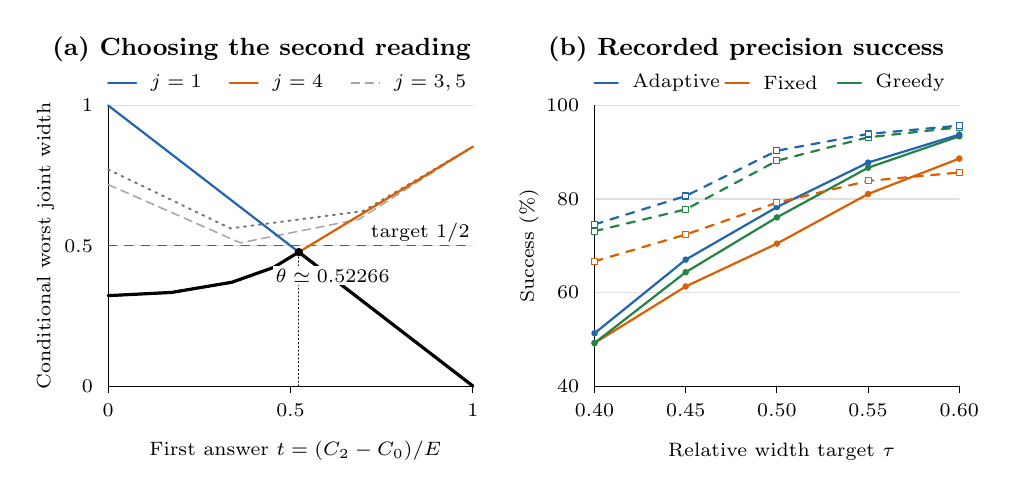
\begin{tikzpicture}[x=0.0098\linewidth,y=0.0098\linewidth,
font=\scriptsize,line cap=round,line join=round]
\definecolor{auditblue}{HTML}{2166AC}
\definecolor{auditorange}{HTML}{D95F02}
\definecolor{auditgreen}{HTML}{238443}
\node[anchor=west,font=\small\bfseries] at (0,47) {(a) Choosing the second reading};
\node[anchor=west,font=\small\bfseries] at (53,47) {(b) Recorded precision success};
\draw (7.000000,11) -- (7.000000,10.3);
\node[anchor=north] at (7.000000,10.1) {0};
\draw (26.500000,11) -- (26.500000,10.3);
\node[anchor=north] at (26.500000,10.1) {0.5};
\draw (46.000000,11) -- (46.000000,10.3);
\node[anchor=north] at (46.000000,10.1) {1};
\draw[black!12] (7,11.000000) -- (46,11.000000);
\node[anchor=east] at (6.4,11.000000) {0};
\draw[black!12] (7,26.000000) -- (46,26.000000);
\node[anchor=east] at (6.4,26.000000) {0.5};
\draw[black!12] (7,41.000000) -- (46,41.000000);
\node[anchor=east] at (6.4,41.000000) {1};
\draw (7,41) -- (7,11) -- (46,11);
\draw[dashed,black!65] (7,26) -- (46,26);
\node[anchor=south east,fill=white,inner sep=1pt] at (46,26) {target $1/2$};
\draw[black!35,densely dashed,line width=.55pt] (7.000000,32.542401) -- (21.137360,26.313235) -- (33.816702,28.829331) -- (46.000000,36.599285);
\draw[black!55,dotted,line width=.7pt] (7.000000,34.157622) -- (20.078835,27.853188) -- (34.270176,29.711230) -- (46.000000,36.599285);
\draw[auditblue,line width=.8pt] (7.000000,41.000000) -- (46.000000,11.000000);
\draw[auditorange,line width=.8pt] (7.000000,20.665739) -- (13.795865,21.011931) -- (20.236979,22.100812) -- (24.663467,23.672268) -- (46.000000,36.599285);
\draw[black,line width=1.15pt] (7.000000,20.665739) -- (13.795865,21.011931) -- (20.236979,22.100812) -- (24.663467,23.672268) -- (27.383609,25.320301) -- (46.000000,11.000000);
\draw[densely dotted] (27.383609,11) -- (27.383609,25.320301);
\fill (27.383609,25.320301) circle[radius=.45];
\node[anchor=north,fill=white,inner sep=1pt] at (31,23.9) {$\theta\simeq0.52266$};
\node[anchor=south] at (27,2) {First answer $t=(C_2-C_0)/E$};
\node[rotate=90] at (0.3,26) {Conditional worst joint width};
\draw[auditblue,line width=.8pt] (7,43.4) -- (10,43.4);
\node[anchor=west] at (10.5,43.4) {$j=1$};
\draw[auditorange,line width=.8pt] (20,43.4) -- (23,43.4);
\node[anchor=west] at (23.5,43.4) {$j=4$};
\draw[black!35,densely dashed] (33,43.4) -- (36,43.4);
\node[anchor=west] at (36.5,43.4) {$j=3,5$};
\draw[black!12] (59,11.000000) -- (98,11.000000);
\node[anchor=east] at (58.4,11.000000) {40};
\draw[black!12] (59,21.000000) -- (98,21.000000);
\node[anchor=east] at (58.4,21.000000) {60};
\draw[black!12] (59,31.000000) -- (98,31.000000);
\node[anchor=east] at (58.4,31.000000) {80};
\draw[black!12] (59,41.000000) -- (98,41.000000);
\node[anchor=east] at (58.4,41.000000) {100};
\draw (59.000000,11) -- (59.000000,10.3);
\node[anchor=north] at (59.000000,10.1) {0.40};
\draw (68.750000,11) -- (68.750000,10.3);
\node[anchor=north] at (68.750000,10.1) {0.45};
\draw (78.500000,11) -- (78.500000,10.3);
\node[anchor=north] at (78.500000,10.1) {0.50};
\draw (88.250000,11) -- (88.250000,10.3);
\node[anchor=north] at (88.250000,10.1) {0.55};
\draw (98.000000,11) -- (98.000000,10.3);
\node[anchor=north] at (98.000000,10.1) {0.60};
\draw (59,41) -- (59,11) -- (98,11);
\draw[auditorange,line width=.8pt] (59.000000,15.603175) -- (68.750000,21.647131) -- (78.500000,26.225885) -- (88.250000,31.537241) -- (98.000000,35.322344);
\fill[auditorange] (59.000000,15.603175) circle[radius=.35];
\fill[auditorange] (68.750000,21.647131) circle[radius=.35];
\fill[auditorange] (78.500000,26.225885) circle[radius=.35];
\fill[auditorange] (88.250000,31.537241) circle[radius=.35];
\fill[auditorange] (98.000000,35.322344) circle[radius=.35];
\draw[auditgreen,line width=.8pt] (59.000000,15.603175) -- (68.750000,23.173382) -- (78.500000,29.034188) -- (88.250000,34.345543) -- (98.000000,37.703297);
\fill[auditgreen] (59.000000,15.603175) circle[radius=.35];
\fill[auditgreen] (68.750000,23.173382) circle[radius=.35];
\fill[auditgreen] (78.500000,29.034188) circle[radius=.35];
\fill[auditgreen] (88.250000,34.345543) circle[radius=.35];
\fill[auditgreen] (98.000000,37.703297) circle[radius=.35];
\draw[auditblue,line width=.8pt] (59.000000,16.641026) -- (68.750000,24.516484) -- (78.500000,30.133089) -- (88.250000,34.894994) -- (98.000000,37.886447);
\fill[auditblue] (59.000000,16.641026) circle[radius=.35];
\fill[auditblue] (68.750000,24.516484) circle[radius=.35];
\fill[auditblue] (78.500000,30.133089) circle[radius=.35];
\fill[auditblue] (88.250000,34.894994) circle[radius=.35];
\fill[auditblue] (98.000000,37.886447) circle[radius=.35];
\draw[auditorange,line width=.8pt,dashed] (59.000000,24.333333) -- (68.750000,27.200717) -- (78.500000,30.605735) -- (88.250000,32.935484) -- (98.000000,33.831541);
\draw[auditorange,fill=white] (58.680000,24.013333) rectangle (59.320000,24.653333);
\draw[auditorange,fill=white] (68.430000,26.880717) rectangle (69.070000,27.520717);
\draw[auditorange,fill=white] (78.180000,30.285735) rectangle (78.820000,30.925735);
\draw[auditorange,fill=white] (87.930000,32.615484) rectangle (88.570000,33.255484);
\draw[auditorange,fill=white] (97.680000,33.511541) rectangle (98.320000,34.151541);
\draw[auditgreen,line width=.8pt,dashed] (59.000000,27.559140) -- (68.750000,29.888889) -- (78.500000,35.086022) -- (88.250000,37.594982) -- (98.000000,38.670251);
\draw[auditgreen,fill=white] (58.680000,27.239140) rectangle (59.320000,27.879140);
\draw[auditgreen,fill=white] (68.430000,29.568889) rectangle (69.070000,30.208889);
\draw[auditgreen,fill=white] (78.180000,34.766022) rectangle (78.820000,35.406022);
\draw[auditgreen,fill=white] (87.930000,37.274982) rectangle (88.570000,37.914982);
\draw[auditgreen,fill=white] (97.680000,38.350251) rectangle (98.320000,38.990251);
\draw[auditblue,line width=.8pt,dashed] (59.000000,28.275986) -- (68.750000,31.322581) -- (78.500000,36.161290) -- (88.250000,37.953405) -- (98.000000,38.849462);
\draw[auditblue,fill=white] (58.680000,27.955986) rectangle (59.320000,28.595986);
\draw[auditblue,fill=white] (68.430000,31.002581) rectangle (69.070000,31.642581);
\draw[auditblue,fill=white] (78.180000,35.841290) rectangle (78.820000,36.481290);
\draw[auditblue,fill=white] (87.930000,37.633405) rectangle (88.570000,38.273405);
\draw[auditblue,fill=white] (97.680000,38.529462) rectangle (98.320000,39.169462);
\node[anchor=south] at (79,2) {Relative width target $\tau$};
\node[rotate=90] at (52,26) {Success (\%)};
\draw[auditblue,line width=.8pt] (59,43.4) -- (61.5,43.4);
\node[anchor=west] at (62,43.4) {Adaptive};
\draw[auditorange,line width=.8pt] (73,43.4) -- (75.5,43.4);
\node[anchor=west] at (76,43.4) {Fixed};
\draw[auditgreen,line width=.8pt] (85,43.4) -- (87.5,43.4);
\node[anchor=west] at (88,43.4) {Greedy};
\end{tikzpicture}
\caption{An acquisition rule and its recorded outcomes. (a) Exact conditional envelopes from the saved HPM~1 comparison on 5 July 2025, 12:00--18:00 UTC, after querying boundary~2. Gray curves show the other second-query options; the black lower envelope selects boundary~4 below the switch and boundary~1 above it. Its maximum is about $0.47734$, below the half-width target for every possible first answer. (b) The adaptive, fixed-batch and greedy policies on all 819 original and 279 external blocks at five reporting targets. Solid curves represent the original panel and dashed curves the external panel. These exploratory recorded success rates use the existing $10^{-8}$ comparison tolerance; they are not worst-case precision probabilities.}
\label{fig:practical-guarantee-replay}
\end{figure}

\FloatBarrier
\subsection{Source panels and audit protocol}
\label{sec:joint-protocol-summary}
We use the first three consumer IDs in the pinned BLEM cumulative-counter
source \citep{blem}. Training covers January--September
2017 and testing October--December 2017. Complete-day and feature filters
leave 91 test days per meter. Hourly energy uses integer counter differences
at exact UTC endpoints, converted to kWh without interpolation; partial days
are excluded. Online Resource~1, S3 records source hashes and fitting details.

The external panel uses HeatpumpMonitor systems 1, 2 and 7
\citep{hpmabout,hpmapi}. We screened ascending IDs for public MID
status, Class-1 electrical-meter metadata and cumulative coverage of
January--July 2025 before hourly retrieval. Training-only gates, fixed
before July retrieval, required 95\% valid hourly intervals
and 90 complete training days. All three passed without replacement.
January--June supplied training; July supplied 31 test days per system.
We convert stored API-grid increments to kWh. Native acquisition and
historical delivery times are unavailable \citep{hpmcode}; S6 records the
source-selection chronology.

Both panels reuse frozen daily-persistence, ridge, boosted-tree and MLP
forecasts. Each external model specification was fitted once without
retuning. We audit blocks ending at 06:00, 12:00 and 18:00 UTC, giving
819 original and 279 external blocks. At each declared cutoff, all policies
receive the endpoints and day-start forecasts; the following day's
persistence copies are not yet available under this benchmark schedule.
Two internal readings serve all six pairs of the four models. This is a
benchmark access contract, not a verified restriction of either source's service;
the public-API experiment also evaluates unrestricted bulk retrieval.
The shared-query analysis is retrospective on both panels. Policies use
frozen forecasts and, for adaptation, previously queried answers. We open
withheld readings only for replay and require $W_r\leq W_{r,0}/2$ for every pair, using the
uncapped exact-total initial widths throughout the shared-query sensitivity controls.
\paragraph{What the measurement model certifies.}
Table~\ref{tab:measurement-assumptions} separates stored-record guarantees
from claims about physical energy. In each mathematical model, the guarantee
requires the unknown record to satisfy the declared constraints.

\begin{table}[htbp]
\centering\small
\caption{Targets and observation assumptions in the application. Error
allowances and hourly caps are sensitivity inputs, not verified device limits.}
\label{tab:measurement-assumptions}
\begin{tabular}{>{\raggedright\arraybackslash}p{0.17\linewidth}>{\raggedright\arraybackslash}p{0.39\linewidth}>{\raggedright\arraybackslash}p{0.34\linewidth}}
\toprule
Model & Target and observations & Scope of the guarantee\\
\midrule
Exact stored samples
& Targets are increments of stored cumulative samples. Retained endpoints
and queried internal samples are exact in this record model.
& Certificates concern loss contrasts on the stored grid. They do not
establish exact physical energy or historical delivery times.\\
Bounded internal errors
& The latent record includes one fixed internal-error vector with
$|e_k|\leq\delta E$, where $E$ is the retained block total. Endpoints, and hence the
retained total, remain exact. Errors are fixed before policy randomization.
& Certificates cover every record and error vector within these bounds.
The $1\%$ allowance is illustrative; it is not sampled noise or device calibration.\\
Physical energy
& Actual energy and meter readings would require defensible bounds for
internal measurements, endpoints and any physical capacity constraints.
& We provide no verified physical calibration. Source meter-class metadata
alone does not establish the pointwise error model or exact endpoints.\\
\bottomrule
\end{tabular}
\end{table}

\paragraph{Unchanged precision under capacity controls.}
For each shared contrast $r$, $W_{r,0}$ remains its initial width under the
original uncapped exact-total model. The shared cap controls retain
$W_r\leq W_{r,0}/2$: they test the same absolute uncertainty budget after
adding hourly information. They do not test halving the new capped initial
width. The scalar control in Online Resource~1, S6 reports both
questions separately. We use the half-width fraction as a declared audit
requirement; it is not a calibrated threshold for a downstream decision.
\begin{table}[htbp]\centering\small
\caption{Numerical conventions for the central shared-query analysis.
Exact certificates and floating-point replay have distinct roles.}
\label{tab:numerical-conventions}
\begin{tabular}{@{}>{\raggedright\arraybackslash}p{.27\linewidth}>{\raggedright\arraybackslash}p{.66\linewidth}@{}}
\toprule
Calculation & Convention\\\midrule
Constructed and matched certificates &
Rational inequalities on the supplied exact inputs; no outcome tolerance.\\
Planner ties and intersections &
Treat values within $10^{-12}$ of a minimum as tied; use the smallest index.
Skip slope differences of magnitude at most $10^{-14}$.\\
Shared mean-batch LP &
Primal and dual feasibility tolerances $10^{-9}$; secondary selection
allows primary objective slack $10^{-10}$.\\
Full-panel floating-point replay &
Classify normalized widths using $J\leq\tau+10^{-8}$.\\
Exact cover replay &
Use exact rational $J\leq\tau$; the exploratory five-threshold analysis
retains both conventions and reports their boundary difference.\\
Printed worked-example coefficients &
The $10^{-4}$ interval is a rational enclosure of displayed coefficients,
not a solver feasibility tolerance. Full coefficients drive the checks.\\
\bottomrule\end{tabular}\end{table}
\section{Results}\label{sec:evaluation}
The application asks which admissible retrieval method meets a required
precision. It separates information available before a query, guarantees
over all compatible records, replay on recorded answers, and actual API
measurements. All policies in each comparison share the same initial
information and measurement model. Scalar readings, network requests and
feedback rounds are different resources. The protocol must identify which
resource is limited before comparing methods.

\subsection{Joint precision with two shared readings}\label{sec:joint-results}
Table~\ref{tab:joint_objectives} separates the planning objectives from
recorded precision success. Table~\ref{tab:joint_precision_status}
identifies where the precision challenger has matching bounds.
\begin{table}[htbp]
\centering\small
\begin{tabular}{>{\raggedright\arraybackslash}p{.19\linewidth}>{\raggedright\arraybackslash}p{.25\linewidth}>{\raggedright\arraybackslash}p{.45\linewidth}}
\toprule
Policy & Planning objective & Guarantee and recorded comparison\\
\midrule
Exact adaptive & Minimize worst joint width & Optimal among deterministic two-query policies in the declared exact model; replay reports joint precision success.\\
Fixed batch & Minimize worst joint width & Best deterministic two-query batch for that width objective; not optimized for recorded success.\\
Greedy adaptive & Myopic first query; optimal continuation & Optimizes the second query after observing the first answer; the first choice need not minimize final worst width.\\
Randomized mean batch & Minimize worst expected joint width & Batch-optimal for the uncapped exact simplex; replay reports expected width and precision success separately.\\
Cover + mean fallback & Certify batch precision success & Globally optimal where lower and upper certificates match; elsewhere uses the mean-width policy, with the remaining probability gap reported.\\
\bottomrule
\end{tabular}
\caption{Objectives are distinct even when all policies share the same two-reading budget, information and query dictionary. Recorded precision success always means $J\leq1/2$; it is neither a minimax success value nor proof that a model winner is identified. The noisy adaptive control freezes an exact-model policy and certifies its guarantees anew, without asserting noisy-policy optimality.}
\label{tab:joint_objectives}
\end{table}

\begin{table}[htbp]
\centering\small
\begin{tabular}{lrrrrrr}
\toprule
Panel & Cases & Closed at 0 & Closed at $1/2$ & Closed at 1 & Open gap & Fallback\\
\midrule
Original & 819 & 141 & 165 & 162 & 351 & 492\\
External & 279 & 27 & 57 & 128 & 67 & 94\\
\bottomrule
\end{tabular}
\caption{Full-panel status of the batch-precision certificates. ``Closed'' means equal certified lower and upper bounds on the continuum batch precision optimum. The three closed columns and open-gap column partition each panel. Fallback is a separate, overlapping policy classification: it includes closed-zero and open-gap instances. Thus 468/819 and 212/279 gaps close, but only the 165 and 57 half-success cases provide the nontrivial $1$-versus-$1/2$ assurance separation.}
\label{tab:joint_precision_status}
\end{table}
\paragraph{Shared-budget evaluation.}
Table~\ref{tab:joint_objectives} distinguishes the five acquisition policies.
The ``closed'' and ``open gap'' labels in Table~\ref{tab:joint_precision_status}
describe whether the lower and upper precision bounds match.
Every method receives the same totals, forecasts and two shared readings
under Section~\ref{sec:joint-protocol-summary}. We set the half-width target
and plan the policies before opening the withheld register responses.
The greedy control first minimizes the worst one-query joint width, breaks
ties using the best two-query continuation, and then minimizes conditional
worst width after the first answer.

\begin{table}[t]
\centering\small
\begin{tabular}{lrrrr}
\toprule
Panel / observation model & Blocks & Adaptive & Fixed batch & Greedy\\
\midrule
Original, exact &819&641 (78.27\%)&577 (70.45\%)&623 (76.07\%)\\
External, exact &279&252 (90.32\%)&221 (79.21\%)&246 (88.17\%)\\
External, $1\%$ allowance &279&242 (86.74\%)&215 (77.06\%)&235 (84.23\%)\\
\bottomrule
\end{tabular}
\caption{Recorded-answer joint precision success with two shared readings.
We select the fixed batch by its worst-width objective before answers;
the last row reoptimizes this comparator for the error model while retaining
the coefficient-derived adaptive and greedy policies. The $1\%$ allowance
enlarges compatible records around the stored answers with exact endpoints,
as defined in Table~\ref{tab:measurement-assumptions}.}
\label{tab:joint_shared_replay}
\end{table}

The adaptive success gains over the best fixed batch for the worst-width objective are
7.81, 11.11 and 9.68 percentage points, respectively. Its gains over greedy
are smaller: 2.20, 2.15 and 2.51 points. For the exact external panel, the
mean realized $J$ is 0.2823 for adaptive, 0.3381 for the fixed batch and
0.2893 for greedy. At the $1\%$ allowance these are 0.3028, 0.3481 and
0.3099. The next comparison uses a batch policy designed for precision.

The cover + mean fallback policy uses a guaranteeing fixed batch when
available, then a certified equal mixture of two batches, and otherwise a
mean-width fallback.
Its recorded success is 54.98\% over the original panel and 72.55\% over the
external panel. These are replay rates for the declared cover and fallback.
Matching certificates prove a batch precision optimum of
$1/2$ on 165 original and 57 external instances. On these instances, adaptive
succeeds on every stored record, while the optimal batch mixtures succeed
with expected frequencies 108/165 (65.45\%) and 37/57 (64.91\%). Coefficient
certificates define these subsets before record replay. The complete fixed-batch and greedy
comparisons in Table~\ref{tab:joint_shared_replay} remain the broader controls.

\paragraph{A stronger guarantee can score worse on stored records.}
Table~\ref{tab:guarantee-recorded-tradeoff} makes the distinction visible on
the same certified subsets. The fixed worst-width batch succeeds more often
on the stored answers than the optimal randomized cover, yet its worst-case
precision success is zero. Indeed, a deterministic batch's worst-case
indicator is either zero or one; a value of one would contradict the
proved randomized optimum of one half. Feedback attains both certainty
over compatible records and success on these recorded cases.

\begin{table}[htbp]\centering\small
\caption{Assurance and replay answer different questions on the matched-half
subsets. Randomized entries are expected success counts for the saved
optimal mixtures. All methods use the same two readings and information.}
\label{tab:guarantee-recorded-tradeoff}
\begin{tabular}{lrrr}\toprule
Policy & Worst-case success & Original (165) & External (57)\\\midrule
Adaptive & $1$ & 165 & 57\\
Fixed worst-width batch & $0$ & 155 & 51\\
Optimal randomized cover & $1/2$ & 108 & 37\\
\bottomrule\end{tabular}\end{table}

\paragraph{Capacity control.}
For an illustrative cap $y_h\leq E/2$, we reoptimize the noiseless planner
using concave piecewise-linear segment widths. We solve each conditional
problem by checking all line intersections within each capacity interval.
Of the 819 original and 279 external records, respectively 780 and 200 satisfy
this cap. Among those compatible records, adaptive-only half-width guarantees
remain in 56 and 4 blocks; recorded adaptive versus fixed-batch successes
are 655 versus 627 and 179 versus 177. Under the stronger cap $E/3$, only
613 original and 198 external records are compatible. No adaptive-only
half-width guarantee remains, and the two planners have equal success counts
of 613 and 192. We restrict cap-based guarantees to compatible records.
Thus supplied capacity information can remove the need for feedback.
Combining the $E/2$ cap with the $1\%$ stored-reading allowance, the
capacity-aware frozen adaptive policy succeeds on 169/200 compatible records,
versus 166/200 for the best fixed batch under that model. Mean joint widths
are 0.3479 and 0.3535. The greedy control succeeds on 165/200 using its
frozen uncapped policy; it has not been reoptimized for the capacity model.

\paragraph{Paired uncertainty and source variation.}
The external exact-panel advantage over the worst-width fixed batch is
11.11 percentage points (descriptive 95\% interval 8.60--13.62), compared
with 2.15 points over greedy (1.08--3.23). These percentile intervals use
2,000 seven-day circular calendar-block resamples, synchronized across the
three systems and intraday blocks, with seed 20261013. The combined cap/error
gain over the fixed batch is 1.50 points ($-0.49$--3.16). Paired $2\times2$
counts, individual-system effects and one-day-cluster sensitivity appear in
Online Resource~1, S8. The intervals describe these panels; three systems
cannot establish population-level generalization, and dependence beyond
the resampled blocks remains unmodeled.
\begin{table}[htbp]
\centering\small
\setlength{\tabcolsep}{4pt}
\begin{tabular}{lrrrrrr}
\toprule
System & $n$ & A / F / G & A-only/F-only & $\Delta_F$ (pp) & A-only/G-only & $\Delta_G$ (pp)\\
\midrule
O1 & 273 & 212/193/211 & 27/8 & 6.96 & 3/2 & 0.37\\
O2 & 273 & 196/187/188 & 30/21 & 3.30 & 9/1 & 2.93\\
O3 & 273 & 233/197/224 & 38/2 & 13.19 & 12/3 & 3.30\\
HPM 1 & 93 & 76/75/73 & 3/2 & 1.08 & 3/0 & 3.23\\
HPM 2 & 93 & 91/66/87 & 25/0 & 26.88 & 4/0 & 4.30\\
HPM 7 & 93 & 85/80/86 & 5/0 & 5.38 & 0/1 & -1.08\\
\bottomrule
\end{tabular}
\caption{Exact-reading paired joint-precision outcomes by system. A is the exact deterministic adaptive planner; F is the best deterministic batch for worst width; G is greedy adaptation. The two discordant counts identify blocks where only A or only its comparator succeeds. O1--O3 are BLEM consumers 1--3; HPM labels retain provider system identifiers. Blocks are repeated observations within systems.}
\label{tab:joint_system_effects}
\end{table}
Table~\ref{tab:joint_system_effects} shows the system-level paired counts.
The external gain over fixed batching is heterogeneous: system~2 supplies
25 of the 31 net additional successes, while system~7 has one fewer success
than greedy adaptation. Omitting each system in turn leaves positive exact-model
panel effects: 5.13--10.07 and 3.23--16.13 percentage points over fixed batching
for the original and external panels, respectively; the corresponding ranges
over greedy are 1.65--3.11 and 1.08--3.76 points. A fourteen-day
synchronized circular-block sensitivity also retains positive exact-model
intervals (Online Resource~1, S8). These checks reuse the same observations;
they are not additional independent replications. The primary seven-day
cap-plus-error interval remains $[-0.49,3.16]$ points. Its fourteen-day
sensitivity is $[0.48,2.63]$, and its leave-one-system-out point effects range
from 0.81 to 2.63 points. This small three-success gain remains sensitive to
the temporal specification; the favorable secondary interval does not replace
the primary assessment.
\paragraph{Checking batch-precision guarantees.}
For each selected batch pair, 36 rational multiplier checks prove that the
two batches cannot both fail on any feasible record. Feasible adverse
records give matching upper bounds, establishing the full-continuum $1/2$
optima. Rational checks also verify the adaptive half-width guarantees.
Elsewhere, we report the gap between the challenger's lower and upper bounds;
the mean-width fallback has only the trivial precision lower bound zero.
Online Resource~1, S8 gives all multipliers, adverse completions and
coefficient-based tie rules. These certificates assume exact readings;
the next calculation treats errors separately.
\paragraph{When feedback changes the available guarantee.}
Exact rational checks partition the original 819 blocks into 162 where a fixed batch guarantees half-width, 168 where adaptive querying does so but no deterministic batch does, and 489 where no deterministic two-query policy does. The corresponding external counts are 128, 57 and 94. These are guarantees over the declared uncapped, noiseless simplex, not frequencies of success on the recorded trace.

Among the 165 original and 57 external blocks with matched randomized-batch optimum $1/2$, the greedy first query fails the half-width requirement on 25 and 13 blocks, respectively, even with its optimal conditional second query. Greedy nevertheless succeeds on the recorded trace in 20 of those 25 and 11 of those 13 blocks. The diagnostic identifies a specific benefit of planning the first query: recorded success can conceal an inadequate pre-query guarantee. Across the full panels, this first-query limitation occurs on 28 and 16 adaptive-guaranteed blocks. The supplied interval covers and uncovered-answer witnesses use rational arithmetic on the stored contrast coefficients.

\paragraph{A stronger fallback check.}
We retain the certified deterministic or equal two-batch cover and replace its mean-width fallback by the fixed worst-width batch on the same 492 original and 94 external fallback blocks. Using the strict threshold $J\leq1/2$, this coefficient-only change raises recorded success from 54.98\% and 72.55\% to 64.71\% and 74.19\%.

Pure fixed batching still performs better (70.45\% and 79.21\%); the entire recorded-score deficit arises on the matched-half subsets, where fixed batching succeeds on 155/165 and 51/57 records, versus expected cover successes of 108/165 and 37/57. On each of those instances, however, every fixed batch has worst-case precision success zero, whereas the cover guarantees $1/2$. The matched-half guarantees and open continuum gaps also apply to this variant. This retrospective diagnostic reuses both panels; the supplement gives both threshold conventions, block-level paired outcomes, system summaries and descriptive seven-day block-bootstrap intervals.
\paragraph{Certifying an insufficient budget.}
Proposition~\ref{prop:assurance-feasibility} closes the last branch of
Figure~\ref{fig:audit-workflow}. All 489 original and 94 external blocks
without a deterministic guarantee have twenty-record certificates bounding
every randomized adaptive policy's success by $19/20<1$. A rational checker
reconstructed all 6,588 source coefficient rows and 5,490 first-query covers,
then verified 11,660 failing endpoint pairs. The smallest strict normalized
failure margins were $0.00031746$ and $0.00073903$, respectively.
These results apply to the uncapped, noiseless model. They justify escalating
an insufficient two-reading contract instead of hoping randomization will
provide certainty. Online Resource~1 includes every synthetic witness; its
default command checks the external panel, and the pinned raw-source route
checks both panels.
\paragraph{How many readings does assurance require?}
The minimum fixed budget is three on every block where two adaptive
readings suffice but two fixed readings do not: 168 original and 57 external
blocks, spanning all six systems. Thus two adaptive readings replace three
necessary and sufficient fixed readings on 225 blocks, a one-third reduction.
Each replacement saves one reading in exchange for an additional information
round: the three fixed readings can be chosen together.
The original count includes the 165 matched-half cases and three further
blocks; only the matched cases establish exact batch success one half.
Using adaptive two on these blocks and the minimum fixed batch elsewhere
gives the complete-panel reading totals in Table~\ref{tab:minimum-reading-budget}.

\begin{table}[htbp]\centering\small
\caption{Reserved optional scalar readings for guaranteed joint half-width
precision. Each plan succeeds for every completion in the declared exact
model. Counts exclude the two common retained endpoints. The adaptive plan
uses a fixed fallback where no two-reading guarantee is available.}
\label{tab:minimum-reading-budget}
\begin{tabular}{lrr}\toprule
Quantity & Original & External\\\midrule
Blocks & 819 & 279\\
Three fixed versus two adaptive & 168 & 57\\
Minimum fixed readings, summed & 2625 & 743\\
Adaptive with fixed fallback, summed & 2457 & 686\\
Reading reduction across full panel & 6.40\% & 7.67\%\\\bottomrule
\end{tabular}
\end{table}

We calculated these budgets from the frozen coefficients before using any
optional reading answers.
Enumeration of all 32 fixed subsets per block agrees with the linear scan.
A separately implemented shortest-path checker verifies minimality and
checks feasible endpoint witnesses and the adaptive interval covers.
Online Resource~1 supplies each concrete fallback batch, source and system
summaries, and the fixed-budget histogram. The capacity and error controls
test how additional information changes the acquisition requirement.
\paragraph{How much remains unresolved in the batch comparison.}
The batch-precision cover has matching continuum bounds on 468 of 819 original
blocks and 212 of 279 external blocks. On the remaining 351 and 67 blocks,
the median upper-minus-lower probability gap is respectively $1/3$ and $1/2$.
The interquartile ranges are $[1/4,1/2]$ and $[1/3,1/2]$; both panels range
from $1/5$ to $1/2$. Averaged over all blocks, including closed gaps, the gaps
are 0.1583 and 0.0983. We use the 165 original and 57 external matched-half certificates as the evidence
of exact precision superiority; the full-panel cover replay is a comparison
with a declared policy, not with a globally solved precision optimum.

\paragraph{Sensitivity to the reporting target.}
Figure~\ref{fig:practical-guarantee-replay}(b) gives an exploratory post-hoc
replay of all 1,098 blocks at relative width targets
$0.40,0.45,0.50,0.55,0.60$, keeping the query policies, fitted models and
mixture parameters fixed.
Across these targets, the adaptive policy's recorded advantage over fixed
batching ranges from 2.08 to 7.81 percentage points on the original panel and
from 7.89 to 11.11 points on the external panel. The advantages over greedy
range from 0.37 to 2.69 and from 0.36 to 2.87 points. Some descriptive
seven-day-block intervals for the greedy comparisons include zero.

\FloatBarrier
\paragraph{Shared-query sensitivity to stored-reading errors.}
Across all 279 external blocks, the frozen shared policy guarantees that
all six normalized comparison widths are at most $1/2$ on 165 blocks under
fixed internal-reading errors bounded by $1\%$ of block energy; the best
deterministic batch does so on 120.  On the 45 additional blocks,
feasible fixed-record certificates prove that every randomized batch has
worst-case precision success below one.  The certified batch success
upper bound has minimum and median $1/2$, interquartile range
$[1/2,2/3]$, and maximum $4/5$; 26 bounds are at most $1/2$ and 37 are
at most $0.7$.  These are upper bounds on the unrestricted batch optimum,
not claims that each bound is attained.  The 45 blocks span all three
external systems (11, 11, and 23 blocks).

Capacity information reduces the benefit.  With a per-hour cap of half
the block energy as well as the same $1\%$ error allowance, a policy
frozen from the capacity-aware noiseless planner certifies 213 of the
279 coefficient instances, versus 204 for the best deterministic batch;
nine have a certified randomized-batch limitation, with upper bounds
between $2/3$ and $7/8$.  Only 200 recorded profiles satisfy this illustrative
cap.  Within that compatible subset the counts are 153 versus 147, with
six separations.  The original uncapped policy certifies only 191 of the
279 capped instances, which motivates using declared capacity information
when planning.  Both policies are fixed before the fine readings are
opened; neither is claimed optimal for bounded-error acquisition.

The comparison uses two shared readings, uncapped noiseless initial widths for
normalization, exact block endpoints, and the same permitted queries for
every method.  A separately implemented rational checker verifies the
saved contrast coefficients, branch coverage, every reported precision
status, and the complete fixed-error adverse records.  Supplementary
methods (Online Resource~1, S8) give the certificate construction.
\paragraph{Reproducibility and numerical checks.}
The supplement connects version-pinned source records, frozen forecasts,
contrast coefficients, saved policies and reported outcomes. A fresh
both-source run reproduced all 1,098 outcome rows exactly, including the
165 original and 57 external matched-half certificates. The original
source route rejects mismatched files; its raw records are regenerated
locally. Default offline replay uses the bundled inputs and is separate
from raw regeneration and fresh model fitting.

A separately written checker reconstructs the policies and summaries. On
18 fixed representative blocks, 19,440 endpoint LPs and 6,480 conditional
LPs have maximum discrepancies of $2.22\times10^{-16}$ and
$1.11\times10^{-16}$, against a $10^{-8}$ check tolerance. Exact rational
covering and adverse-record inequalities establish the matched precision
claims. An optimal-face diagnostic also checks that arbitrary selection
among mean-optimal batch mixtures does not explain their lower recorded
success. Online Resource~1, S8 supplies the full checks and the
results-to-command map identifies each reproduction entry point.
\subsection{What the retrieval interface changes}
\label{sec:actual-api}
The HeatpumpMonitor API permits full-range retrieval, so we tested it
directly \citep{hpmapi,hpmcode}. We fixed the first eligible
daily-persistence--MLP task from each external system before querying its
optional answers. Two repetitions of five policies produced 30 trials
and 60 HTTP requests, including common endpoint reads.

\begin{table}[htbp]\centering\small
\caption{Observed public-API control: three tasks, two repetitions per
policy. Incremental I/O excludes client throttle waiting. The full-range
response contains seven hourly samples, including five internal readings.
All five tested policies met the precision
target; the full five-policy measurements and cached response hashes are
in Online Resource~1, S15.}\label{tab:actual-api}
\begin{tabular}{lrrr}\toprule
Policy & Requests & Mean I/O (s) & Mean body bytes\\\midrule
Exact adaptive & 2 & 0.497 & 104.3\\
Full hourly range & 1 & 0.331 & 226.7\\\bottomrule
\end{tabular}\end{table}

Bulk retrieval uses one request, achieves zero terminal width and has
lower observed I/O time on these tasks. We therefore recommend bulk when
the full response is admissible. For selective access, the minimum-budget
calculation identifies the readings needed for assurance and the possible
reduction from feedback. Online Resource~1, S8 supplies the protocol selector
and its reading and acquisition-round cost catalogue.
\section{Discussion}
\subsection{Planning the readings needed for assurance}
The auditor supplies the comparisons, available information and permissible
measurements. Our method returns the minimum sufficient fixed reading budget
and checks whether feedback reduces it. On 168 original and 57 external
blocks, three fixed readings are necessary and sufficient, while two adaptive
readings suffice. Each saving exchanges one scalar reading for an additional
information round. This calculation lets the auditor compare plans before
opening the optional measurements.

Theorem~\ref{thm:two-target-collapse} explains why sharing readings matters.
Two simultaneous comparisons can remove the scalar two-query success floor:
adaptive certainty coexists with optimal batch success $1/m$, although each
contrast separately admits a sufficient fixed batch. The adverse records
force all $m$ batches even for positive worst-record success and identify the
unique optimal mixture. The output dimension and query budget stay fixed as
the dictionary grows; three fixed readings suffice in this construction.

The meter study connects this distinction to frozen forecast geometries.
With two readings shared across six comparisons, 165 original and 57
external blocks have adaptive success one and optimal batch success one
half. The worked example reports both normalized widths and original loss
units (Table~\ref{tab:absolute_joint_widths}). On recorded answers, joint
precision gains are 7.81 and 11.11 percentage points over fixed worst-width
batching and 2.20 and 2.15 over greedy adaptation. Separate-pair gains are
0.407 and 0.119 points.

\subsection{Scope and protocol choice}
These guarantees apply to the specified information and query dictionary.
The main planner uses two cumulative-prefix queries and an exact
nonnegative total. The minimum-budget result counts scalar readings;
the API control measures requests and I/O time. Bulk retrieval wins on that
three-task workload: one request returns the complete record faster and
leaves zero width. A selective plan is therefore relevant when the auditor
limits individual readings; an admissible full-record export favors bulk.
The source panels do not establish a deployed selective-access service.

Additional information can change the plan. The stronger $E/3$ capacity
control removes the adaptive-only half-width advantage on compatible
records. Bounded errors can increase the sufficient reading budget.
Table~\ref{tab:measurement-assumptions} states these sensitivity models,
including exact retained endpoints and uncalibrated error allowances.
The source panels each contain three systems and were reused retrospectively.
Matching certificates establish the exact batch optima on the reported
subsets; 351 original and 67 external full-panel precision gaps remain open.

Precision is a reporting requirement; model selection also depends on the
intervals' positions. On the external panel, adaptation certifies a best
model on 207 blocks and greedy on 208. Original counts are 123 and 118;
fixed batches certify 122 original and 201 external blocks. Thus the
half-width criterion measures reliable comparison precision, with winner
certification reported as a separate outcome. Online Resource~1 contains the
broader scalar theory, coordinate-recovery solver and protocol-selection
cost sensitivity. A next step is to develop scalable planners for larger
adaptive reading budgets.

\section{Conclusions}
Sharing a reading budget can make feedback necessary for an assurance
requirement that each comparison can meet separately. With two affine
targets and two coordinate queries, adaptive success can be one while
optimal randomized-batch success is $1/m$. The same construction covers
all pairs among three models.

Our exact planner and verifiable certificates turn this boundary into a
reading-budget decision. On 225 blocks across six systems, two adaptive
readings replace the minimum three fixed readings; 222 also have matching
batch-success bounds of one half. Combining these adaptive plans with
minimum fixed batches elsewhere reduces reserved readings by 6.40\% and
7.67\% across the original and external panels under the exact-total model.
The resulting plans specify the readings and feedback needed to attain a
stated assurance level, allowing an auditor to select a protocol that fits
the available access interface.
\section*{Supplementary Materials}
Online Resource 1 is supplied as Supplemental Data S1 and S2. Extract both
ZIP files into the same directory. Together they contain the editable
manuscript, executable methods, frozen forecasts, source identifiers, case
ledgers, exact witnesses and numerical checks. Start with \texttt{README.txt};
\texttt{CURRENT\_RESULTS\_MAP.txt} maps each current table and verification
claim to its command, inputs and outputs. The default verification replays
saved forecasts and does not train new models. Separate commands cover
raw-input regeneration and fresh fitting. BLEM-derived traces are reconstructed
locally; attributed HeatpumpMonitor records are bundled. The indexed extended
methods retain full proofs, solver scaling, historical controls, forecasting
protocols and uncertainty checks. Protocol-selection files include all 116
interface decisions and task-bound readout checks. The separate checker
compares saved contrasts with frozen geometry, verifies forecast hashes,
and reconstructs retained endpoints from cached API records. Historical
reports relevant to this revision are retained; the larger development
archive is preserved separately.

\section*{Additional Information and Declarations}
\subsection*{Data and Code Availability}
The numerical code and detailed outputs are supplied in Online Resource 1.
The public source identifiers are given in the references. The package
separates bundled Portugal/household replay from BLEM raw-source
regeneration. BLEM counter traces are regenerated from the pinned public
QuantLet repository (\url{https://github.com/QuantLet/BLEM}), accompanying
Kostmann and H\"ardle (2019; \url{https://doi.org/10.3390/en12142718}).
The regeneration commands reject inputs with mismatched hashes.
These raw traces are not redistributed because redistribution permission
has not been established.
Constructed polytopes include their complete inequalities and objectives.
Dual outputs retain raw multipliers, any numerical mass correction, the
completed record, and pricing and enumerated lower bounds. LP and endpoint
cross-checks use floating-point arithmetic with explicit tolerances; the
counter covering and adverse-profile certificates are additionally checked
with exact rational arithmetic on their serialized inputs. Shared-query
checks include all joint outcomes, optimal-batch tie diagnostics, bounded-error
dual certificates and adverse completions. Reviewers receive the current
executable materials as Supplemental Data S1 and S2.

\subsection*{Funding}
This research received no external funding.

\subsection*{Competing Interests}
The author declares no competing interests.

\subsection*{Author Contributions}
Jishan Kapoor defined the research objectives and evaluation requirements,
directed and supervised the analysis and revisions, interpreted the findings,
and approved the manuscript. The computational and drafting assistance used
under this supervision is described below.

\subsection*{Research Transparency}
This work uses public data and constructed mathematical instances, with
no newly recruited participants. New measurements concern public API
response times and payloads, with their small-workload scope reported. Retrospective masks and
archive-access assumptions are identified explicitly. Comparisons use
the same information and the same stated hard budgets. The new proofs
and numerical checks do not change the historical forecast results.

\section*{Acknowledgements}
\paragraph{Generative-AI assistance.}
Jishan Kapoor provided the topic, set the research objectives and evaluation
requirements, directed the analyses and tests, and closely supervised all
use of OpenAI Codex (OpenAI; GPT-6-family assistant for the final revision;
accessed October 2026; exact model identifiers for earlier sessions were
not consistently retained). The tool assisted with literature searches,
development and checking of research content and code, computational
execution, and manuscript drafting and editing. It supported iterative
verification and clearer presentation. The author reviewed and revised
these outputs, checked the tools' terms of use and confirmed their suitability
for publishing this work. The author retains full responsibility for the
research decisions, originality and integrity of the work, accuracy of the
references, interpretation of results, and final manuscript. Separate checker
implementations within this study are not external independent replication.
This generative assistance is distinct from the boosted-tree and neural
forecasting models fitted to the public application data.


\FloatBarrier
\begin{thebibliography}{99}
\bibitem[Amenta et~al.(2016)]{amenta2016}
Amenta, N., De Loera, J. A., \& Sober\'on, P. (2016). Helly's theorem: new variations
and applications. Author manuscript, arXiv:1508.07606v2.
\url{https://arxiv.org/abs/1508.07606v2}

\bibitem[Gaillard et~al.(2023)]{gaillard2023}
Gaillard, P., Gerchinovitz, S., \& de Montbrun, {\'E}. (2023).
Adaptive approximation of monotone functions [Preprint].
arXiv. \url{https://arxiv.org/abs/2309.07530v1}

\bibitem[Hara et~al.(2024)]{hara}
Hara, S., Matsuura, M., Honda, J., \& Ito, S. (2024).
Active model selection: A variance minimization approach.
\emph{Machine Learning, 113}, 8327--8345.
\url{https://doi.org/10.1007/s10994-024-06603-1}

\bibitem[Iancu and Trichakis(2014)]{iancu2014}
Iancu, D. A., \& Trichakis, N. (2014). Pareto efficiency in robust optimization.
\emph{Management Science, 60}(1), 130--147.
\url{https://doi.org/10.1287/mnsc.2013.1753}

\bibitem[Kawase and Sumita(2024)]{kawase2024}
Kawase, Y., \& Sumita, H. (2024). Randomized strategies for robust
combinatorial optimization with approximate separation.
\emph{Algorithmica, 86}, 566--584.
\url{https://doi.org/10.1007/s00453-023-01175-3}

\bibitem[Kossen et~al.(2021)]{active}
Kossen, J., Farquhar, S., Gal, Y., \& Rainforth, T. (2021).
Active testing: Sample-efficient model evaluation.
\emph{Proceedings of Machine Learning Research, 139}, 5753--5763.
\url{https://proceedings.mlr.press/v139/kossen21a.html}

\bibitem[Kostmann and H\"ardle(2019)]{blem}
Kostmann, M., \& H\"ardle, W. K. (2019). Forecasting in blockchain-based
local energy markets. \emph{Energies, 12}, 2718.
\url{https://doi.org/10.3390/en12142718}
Source data: \url{https://github.com/QuantLet/BLEM}.

\bibitem[Krieg et~al.(2025)]{krieg2025}
Krieg, D., Novak, E., \& Ullrich, M. (2025).
On the power of adaption and randomization.
\emph{Forum of Mathematics, Sigma, 13}, e152.
\url{https://doi.org/10.1017/fms.2025.10101}

\bibitem[Krieg and Ullrich(2026)]{krieg2026}
Krieg, D., \& Ullrich, M. (2026).
Approximation of functions: Optimal sampling and complexity.
\emph{Acta Numerica, 35}, 273--457.
\url{https://doi.org/10.1017/S0962492925100287}
Author manuscript: \url{https://arxiv.org/abs/2602.02066v2};
section and equation locators in the text refer to that version.

\bibitem[Kuboyama(2026)]{kuboyama2026}
Kuboyama, T. (2026).
How many labels does model choice need? Certificates and budgets for selective
prediction [Preprint].
arXiv. \url{https://arxiv.org/abs/2609.18622v1}

\bibitem[Kurtz(2026)]{kurtz2026}
Kurtz, J. (2026). Bounding the optimal number of policies for robust
K-Adaptability. \emph{Mathematical Programming}. Published 29 January 2026.
\url{https://doi.org/10.1007/s10107-026-02329-1}

\bibitem[Maia Polo et~al.(2024)]{polo}
Maia Polo, F., Maity, S., Yurochkin, M., Banerjee, M., \& Sun, Y. (2024).
Weak supervision performance evaluation via partial identification.
\emph{Advances in Neural Information Processing Systems, 37}.
\url{https://doi.org/10.52202/079017-4309}

\bibitem[Manski(2005)]{manski}
Manski, C. F. (2005). Partial identification with missing data:
Concepts and findings. \emph{International Journal of Approximate
Reasoning, 39}, 151--165.
\url{https://doi.org/10.1016/j.ijar.2004.10.006}

\bibitem[Martin et~al.(1990)]{martin1990}
Martin, R. K., Rardin, R. L., \& Campbell, B. A. (1990).
Polyhedral characterization of discrete dynamic programming.
\emph{Operations Research, 38}(1), 127--138.
\url{https://doi.org/10.1287/opre.38.1.127}

\bibitem[Novak(1995)]{novak1995}
Novak, E. (1995). The adaption problem for nonsymmetric convex sets.
\emph{Journal of Approximation Theory, 82}(1), 123--134.
\url{https://doi.org/10.1006/jath.1995.1071}

\bibitem[Novak and Wo{\'z}niakowski(2008)]{novak2008}
Novak, E., \& Wo{\'z}niakowski, H. (2008).
\emph{Tractability of multivariate problems. Volume I: Linear information}.
European Mathematical Society.
\url{https://doi.org/10.4171/026}

\bibitem[Okanovic et~al.(2025)]{okanovic2025}
Okanovic, P., Kirsch, A., Kasper, J., Hoefler, T., Krause, A., \&
G\"urel, N. M. (2025). All models are wrong, some are useful:
Model selection with limited labels.
\emph{Proceedings of Machine Learning Research, 258}, 2035--2043.
\url{https://proceedings.mlr.press/v258/okanovic25a.html}

\bibitem[OpenEnergyMonitor(2026a)]{hpmabout}
OpenEnergyMonitor. (2026a). HeatpumpMonitor.org: About.
\url{https://heatpumpmonitor.org/about}. Accessed 12 October 2026.

\bibitem[OpenEnergyMonitor(2026b)]{hpmapi}
OpenEnergyMonitor. (2026b). HeatpumpMonitor.org API helper.
\url{https://heatpumpmonitor.org/api-helper}. Accessed 12 October 2026.

\bibitem[OpenEnergyMonitor(2026c)]{hpmcode}
OpenEnergyMonitor. (2026c). HeatpumpMonitor.org timeseries controller and
Emoncms PHPTimeSeries implementation. Source snapshots and hashes supplied
in Online Resource 1.
\url{https://github.com/openenergymonitor/heatpumpmonitor.org/blob/main/www/Modules/timeseries/timeseries_controller.php};
\url{https://github.com/openenergymonitor/emoncms/blob/master/Modules/feed/engine/PHPTimeSeries.php}.
Accessed 12 October 2026.

\bibitem[Osipenko(2019)]{osipenko}
Osipenko, K. Yu. (2019). Generalized adaptive versus nonadaptive recovery
from noisy information. \emph{Journal of Complexity, 53}, 162--172.
\url{https://doi.org/10.1016/j.jco.2018.12.001}

\bibitem[Patton(2011)]{patton}
Patton, A. J. (2011). Volatility forecast comparison using imperfect
volatility proxies. \emph{Journal of Econometrics, 160}(1), 246--256.
\url{https://doi.org/10.1016/j.jeconom.2010.03.034}

\bibitem[Sawade et~al.(2012)]{sawade}
Sawade, C., Landwehr, N., \& Scheffer, T. (2012).
Active comparison of prediction models.
\emph{Advances in Neural Information Processing Systems, 25}.
\url{https://proceedings.neurips.cc/paper_files/paper/2012/file/92fb0c6d1758261f10d052e6e2c1123c-Paper.pdf}

\bibitem[Sion(1958)]{sion1958}
Sion, M. (1958). On general minimax theorems.
\emph{Pacific Journal of Mathematics, 8}(1), 171--176.
\url{https://doi.org/10.2140/pjm.1958.8.171}

\bibitem[Vayanos et~al.(2026)]{ddid}
Vayanos, P., Georghiou, A., \& Yu, H. (2026).
Robust optimization with decision-dependent information discovery.
\emph{Management Science, 72}(2), 1509--1528.
\url{https://doi.org/10.1287/mnsc.2021.00160}

\bibitem[Wei and Zhang(2024)]{wei2024}
Wei, N., \& Zhang, P. (2024). Adjustability in robust linear optimization.
\emph{Mathematical Programming, 208}, 581--628.
\url{https://doi.org/10.1007/s10107-023-02049-w}
% New entries; place Gaillard before Hara and Kuboyama after Krieg in the
% alphabetized bibliography. Existing wei2024 and ddid entries are reused.
\end{thebibliography}
\end{document}
